\documentclass[tp]{lcc}

% add latex preamble
% para la bibliografía se requiere biber y configurar texstudio

% Latex packages
\usepackage[utf8]{inputenc}
\usepackage[T1]{fontenc} % para copiar acentos en español del pdf y permite acentos en las notas
\usepackage[spanish]{babel}
\usepackage[per-mode = symbol]{siunitx} % para manejar las unidades
\usepackage{multimedia} % to add videos with \movie command
\usepackage{multirow}
\usepackage{graphicx}
\usepackage{xcolor}
\usepackage{amsmath} % bmatrix
\usepackage[makeroom]{cancel} % \cancel to cancel terms in math equations
\renewcommand{\CancelColor}{\color{red}} % set red color for \cancel command
\usepackage[caption=false]{subfig} % caption = false elimina la palabra "Figura" del caption
\usepackage{import} % para el comando import (se usa para pdf_tex)
\captionsetup[subfigure]{labelformat=empty} % remover el indice del caption de la subfigura
\usepackage{booktabs} % \toprule \midrule \bottomrule
\usepackage[backend=biber]{biblatex} % set biber to format references. Must configure Biber in Texstudio
\usepackage{csquotes} % to remove warning triggered by biblatex and babel
\usepackage{algorithm} % to put captions to the algorithmics environmets
\usepackage{algpseudocode} % to write algorithm
\usepackage{tikz} % to use tikz
\usetikzlibrary{fit} % to fit a node around other nodes in tikz
\usepackage[export]{adjustbox} % valign in subfloat
\usepackage{colortbl} % to paint cells in a table

% Color commands for annotations
\newcommand\TODO[1]{\textbf{\textcolor{red}{#1}}} %  TODO notes

% Graphic paths
\graphicspath{{./images/}}

% listings configuration for C code
\usepackage{listings} % code
\definecolor{commentgreen}{RGB}{2,112,10}
\definecolor{eminence}{RGB}{108,48,130}
\definecolor{weborange}{RGB}{255,165,0}
\definecolor{frenchplum}{RGB}{129,20,83}

\lstset{ % spanish characters for listings package
	inputencoding=latin1,
    columns=fullflexible,
	breaklines=true,
	tabsize=2,
	showstringspaces=false,
	basicstyle=\ttfamily,
	backgroundcolor=\color{lightgray}, % Choose background color
	literate={á}{{\'a}}1
	{ã}{{\~a}}1
	{é}{{\'e}}1
	{ó}{{\'o}}1
	{í}{{\'i}}1
	{ñ}{{\~n}}1
	{¡}{{!`}}1
	{¿}{{?`}}1
	{ú}{{\'u}}1
	{Í}{{\'I}}1
	{Ó}{{\'O}}1
    {-}{-}1
}

\lstdefinestyle{cpp}{ % spanish characters for listings package
    language=C++,
   	commentstyle=\color{commentgreen},
    keywordstyle=\color{eminence},
    stringstyle=\color{red},
    emph={int,char,double,float,unsigned,void,bool},
    emphstyle={\color{blue}}
}

\lstdefinestyle{bash}{ % spanish characters for listings package
	language=Bash
}

\lstdefinestyle{xml}{
	language=XML,
	morekeywords={encoding,xs:schema,xs:element,xs:complexType,xs:sequence,xs:attribute}
}

\lstdefinestyle{cmake}{
	language=make, % there is no cmake support in listings
}

\lstdefinestyle{python}{
    language=python,
}


%%%%% PARA QUE EN LAS TABLAS SE PUEDA PONER UN SALTO DE LINEA DENTRO DE UNA CELDA
\newcommand{\specialcell}[2][c]{%
    \begin{tiny}
        \begin{tabular}[#1]{@{}c@{}}#2\end{tabular}  
    \end{tiny}
}
%%%%%%%%%%%%%%%%%%%%%%%%%%%%%%%%%%%%%%%%%%%%%%%%%%%%%%%%%%%%%%%%%%%%%%%%

%%%%% PARA QUE LAS TABLAS TENGAN TODAS LAS COLUMNAS CENTRADAS Y DE IGUAL TAMAÑO
\usepackage{tabularx}
\renewcommand{\tabularxcolumn}[1]{>{\centering\arraybackslash}m{#1}}
%%%%%%%%%%%%%%%%%%%%%%%%%%%%%%%%%%%%%%%%%%%%%%%%%%%%%%%%%%%%%%%%%%%%%%%%



% add math preamble
\usepackage{amsmath}
\usepackage{amssymb}
\usepackage{amsopn}
\usepackage{mathtools}

% math
\renewcommand{\vec}[1]{\boldsymbol{\mathbf{#1}}}
\newcommand{\norm}[1]{\lVert#1\rVert}

% Declare arg max and arg min functionss
\DeclareMathOperator*{\argmax}{arg\,max}
\DeclareMathOperator*{\argmin}{arg\,min}

% Homogeneous decoration function
\newcommand{\homo}[1]{\dot{#1}}


% Declare projection as math function
\DeclareMathOperator{\proj}{proj}
\newcommand{\fromCoord}[2]{{#1}_\mathrm{#2}}
\newcommand{\toCoord}[2]{\prescript{\mathrm{#2}}{}{#1}}
\newcommand{\worldCoordSystem}{\mathrm{w}}
\newcommand{\bodyCoordSystem}{\mathrm{B}}
\newcommand{\cameraCoordSystem}{\mathrm{c}}
\newcommand{\point}{\vec{p}}
\newcommand{\worldPoint}{\toCoord{\point}{\worldCoordSystem}}
\newcommand{\imagePoint}{\vec{u}}
\newcommand{\cameraPoint}{\toCoord{\point}{\cameraCoordSystem}}
\newcommand{\homoWorldPoint}{\toCoord{\homo{\point}}{\worldCoordSystem}}
\newcommand{\homoImagePoint}{\homo{\imagePoint}}
\newcommand{\homoCameraPoint}{\toCoord{\homo{\point}}{\cameraCoordSystem}}
\newcommand{\measurement}{\vec{z}}
\newcommand{\prediction}{\hat{\vec{z}}}
\newcommand{\seMatrix}{\vec{\xi}}
\newcommand{\transform}[2]{\toCoord{\fromCoord{\seMatrix}{#2}}{#1}}
\newcommand{\pointCoord}[1]{\toCoord{\point}{#1}}
\newcommand{\rotation}{\vec{R}}
\newcommand{\rotationCoord}[2]{\toCoord{\fromCoord{\rotation}{#2}}{#1}}
\newcommand{\translation}{\vec{t}}
\newcommand{\translationCoord}[2]{\toCoord{\fromCoord{\translation}{#2}}{#1}}
\newcommand{\intrinsicMatrix}{\vec{K}}
\newcommand{\principalPoint}{\vec{c}}
\newcommand{\reprojectionError}{u}
\newcommand{\projectionMatrix}{\vec{P}}
\newcommand{\cameraCenter}{\vec{o}}
\newcommand{\essentialMatrix}{\vec{E}}
\newcommand{\inverse}[1]{{#1}^{-1}}

% Motion model
\newcommand{\position}{\vec{p}}
\newcommand{\orientationQuaternion}{\vec{q}}
\newcommand{\predictedPosition}{\hat{\vec{p}}}
\newcommand{\predictedOrientationQuaternion}{\hat{\vec{q}}}
\newcommand{\linearVelocity}{\vec{v}}
\newcommand{\angularVelocity}{\vec{\omega}}

\DeclareMathOperator{\slerpOp}{slerp}
\newcommand{\slerp}[1]{\slerpOp{\left( #1 \right)}}

% Map structure
\newcommand{\map}{M}
\newcommand{\keyframesSet}{K}
\newcommand{\mapPointsSet}{P}
\newcommand{\observedMapPoints}{O}
\newcommand{\covisibilityKeyframes}{CK}
\newcommand{\localMap}{local\_map}



% Bundle Adjutment
\newcommand{\update}{\vec{\delta}}
\newcommand{\incremental}{\hat{\update}}


% Loop Closure names

% scaled operators and letters to fancy view
\newcommand{\sminus}{\scalebox{0.5}[1.0]{$-$}}
\newcommand{\splus}{\scalebox{0.6}[0.6]{$+$}}
\newcommand{\curr}{c}
\newcommand{\sind}[1]{\scalebox{0.6}[0.6]{$#1$}}
\newcommand{\ind}[1]{\scalebox{0.7}[0.7]{$#1$}}

\newcommand{\keyframe}{\vec{K}}
\newcommand{\bowVector}{\vec{v}}
\newcommand{\lcError}{\vec{\Omega}}
\newcommand{\relativeTransformation}{\seMatrix}
\DeclareMathOperator{\interpolate}{interpolate}

\newcommand{\relativeMotion}{\vec{\delta}}
\newcommand{\groundTruth}[1]{{#1}^{*}}



% definición del operador rot()
\DeclareMathOperator{\rotationOp}{rot}
\newcommand{\getRotation}[1]{\rotationOp{\left( #1 \right)}}

\DeclareMathOperator{\translationOp}{trans}
\newcommand{\getTranslation}[1]{\translationOp{\left( #1 \right)}}









\codigo{R-521}
\materia{Robótica Móvil}
\titulo{EKF y PF para Localización de un Robot Móvil}

\soluciones
\commentstrue


\usepackage{biblatex}
%\addbibresource{refs.bib}

\begin{document}
	\maketitle
	
	
	\section{Introducción}
	
	El objetivo del Trabajo Práctico es comprender cómo funciona el Filtro de Kalman Extendido (EKF) y el Filtro de Partículas (PF) para la localización de un robot móvil y desarrollar una implementación de cada uno.
	
	Para este trabajo se utilizará el framework de Python provisto por la cátedra. Sin embargo, se alienta a que el trabajo se desarrolle utilizando ROS2 y Gazebo. \footnote{Este trabajo práctico está basado en el Homework 2 del curso CSE571: Probabilistic Robotics of University of Washington - Paul G. Allen School of Computer Science \& Engineering \url{https://courses.cs.washington.edu/courses/cse571/20sp/homeworks/HW2.pdf}.}
	
	Material de lectura útil: slides de las clases, Capítulos 3, 4, 5, 7 y 8 del libro Probabilistic Robotics, Thrun, Burgard and Fox.
	
	
	\section{Entrega}
	\begin{itemize}
		\item Se debe proveer un repositorio git que contenga el código desarrollado, una imagen docker y un archivo \lstinline{README.md} con las instrucciones de compilación y ejecución.
		
		\item Se debe entregar un informe en Lyx o \LaTeX\  explicando el trabajo realizado y analizando los resultados obtenidos.
	\end{itemize}

	
	\section{Ejercicios Teóricos}
    
    \ejercicio Kalman Gain
    
    Recordemos que si tenemos dos funciones de densidad de probabilidad Gaussianas:
    
    \begin{align*}
        f(x) &= \mathcal{N}(x;\mu_{1},\sigma_{1}^{2})\\
        g(x) &= \mathcal{N}(x;\mu_{2},\sigma_{2}^{2})
    \end{align*}
%
    Entonces, su producto es una Gaussiana (a un factor de escala):
%
    \begin{equation*}
        f(x)g(x) \propto \mathcal{N} \left(x; \dfrac{\sigma_{2}^{2}}{\sigma_{1}^{2} + \sigma_{2}^{2}}\mu_{1} + \dfrac{\sigma_{1}^{2}}{\sigma_{1}^{2} + \sigma_{2}^{2}}\mu_{2}, \dfrac{1}{\sigma_{1}^{-2} + \sigma_{2}^{-2}} \right)
    \end{equation*}

    Demuestre que en 1D, el paso de corrección del Filtro de Kalman que se muestra a continuación es equivalente (hasta un factor de escala) a la multiplicación de las Gaussianas del estado predicho ($\mathcal{N}(x;\overline{\mu}_{1},\overline{\sigma}_{1}^{2})$) y de observación ($\mathcal{N}(z;x, \sigma_{obs}^{2})$) con media y varianza dadas por:
    
    \begin{align*}
        \mu &= \overline{\mu} + K (z - \overline{\mu})\\
        \sigma^{2} &= (1 - K) \overline{\sigma}^{2}
    \end{align*}
%
    donde 
    \begin{equation*}
        K = \dfrac{\overline{\sigma}^{2}}{\overline{\sigma}^{2}+\sigma_{obs}^{2}}.
    \end{equation*}
	
	\ejercicio Jacobiano del Modelo de Movimiento
    \label{exercise:jacobian}
    
    La Figura~\ref{fig:odometry-base-motion-model} describe un modelo de movimiento simple. El estado del robot es su posición y orientación 2D: $s = [x, y, \theta]$. El control del robot es $\controlCommand = [\delta_{rot1}, \delta_{trans}, \delta_{rot2}]$, es decir el robot rota $\delta_{rot1}$, se desplaza $\delta_{trans}$ y luego rota $\delta_{rot2}$.
    
    Las ecuaciones para el modelo de movimiento $g$ son las siguientes:
    
    \begin{align*}
        x_{t+1} &= x_{t} + \delta_{trans} \cos(\theta_{t} + \delta_{rot1})\\
        y_{t+1} &= y_{t} + \delta_{trans} \sin(\theta_{t} + \delta_{rot1})\\
        \theta_{t+1} &= \theta_{t} + \delta_{rot1} + \delta_{rot2}
    \end{align*}

    donde $s_{t+1} = [x_{t+1}, y_{t+1}, \theta_{t+1}]$ es la predicción del modelo de movimiento. Derivar los Jacobianos de $g$ respecto del estado $\motionModelJacobian = \dfrac{\partial g}{\partial s}$ y el control $\motionModelJacobianControl = \dfrac{\partial g}{\partial \controlCommand}$
    
    \noindent
    \begin{minipage}[t]{.5\textwidth}
    \begin{equation*}
        \motionModelJacobian =
        \begin{bmatrix}
            \dfrac{\partial x^{\prime}}{\partial x} & \dfrac{\partial x^{\prime}}{\partial y} & \dfrac{\partial x^{\prime}}{\partial \theta}\\
            \dfrac{\partial y^{\prime}}{\partial x} & \dfrac{\partial y^{\prime}}{\partial y} & \dfrac{\partial y^{\prime}}{\partial \theta}\\
            \dfrac{\partial \theta^{\prime}}{\partial x} & \dfrac{\partial \theta^{\prime}}{\partial y} & \dfrac{\partial \theta^{\prime}}{\partial \theta}
        \end{bmatrix}
\end{equation*}
    \end{minipage}% <---------------- Note the use of "%"
    \begin{minipage}[t]{.5\textwidth}
        \begin{equation*}
            \motionModelJacobianControl =
            \begin{bmatrix}
                \dfrac{\partial x^{\prime}}{\partial \delta_{rot1}} & \dfrac{\partial x^{\prime}}{\partial \delta_{trans}} & \dfrac{\partial x^{\prime}}{\partial \delta_{rot2}}\\
                \dfrac{\partial y^{\prime}}{\partial \delta_{rot1}} & \dfrac{\partial y^{\prime}}{\partial \delta_{trans}} & \dfrac{\partial y^{\prime}}{\partial \delta_{rot2}}\\
                \dfrac{\partial \theta^{\prime}}{\partial \delta_{rot1}} & \dfrac{\partial \theta^{\prime}}{\partial \delta_{trans}} & \dfrac{\partial \theta^{\prime}}{\partial \delta_{rot2}}
            \end{bmatrix}
        \end{equation*}
    \end{minipage}
    
	
	\section{Ejercicios de Programación}
		
	Implementar un Filtro de Kalman Extendido (EKF) y un Filtro de Partículas (PF) para localizar un robot utilizando \emph{landmarks}. Usaremos el modelo de movimiento basado en la odometría que se derivó previamente. Asumimos que hay landmarks presentes en el entorno del robot. El robot recibe los ángulos (\emph{bearing}) a los landmarks y los ID de los landmarks como observaciones: (orientación, ID de landmark).
	
	Asumimos un modelo de ruido para el modelo de movimiento de odometría con parámetro $\alpha$ (ver Libro Probabilisitc Robotics Tabla 5.6) y un modelo de ruido separado para las observaciones de ángulo con parámetro $\beta$ (ver Libro Probabilisitc Robotics Sección 6.6). El ID del landmark en las observaciones es sin ruido. Consulte el código provisto para obtener detalles de implementación.
	
	En cada paso de tiempo, el robot comienza desde el estado actual y se mueve de acuerdo con la entrada de control. El robot luego recibe una observación del mundo. Utilizar esta información para localizar el robot sobre la secuencia de tiempo completa con un EKF y PF.
	
	\begin{figure}[!htbp]
		\centering
		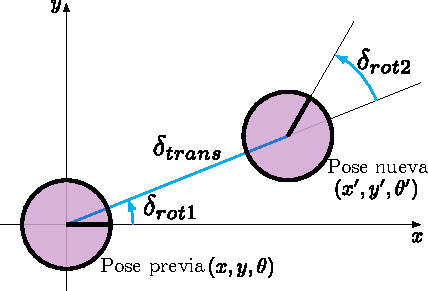
\includegraphics[width=0.5\textwidth]{./images/odometry_as_controls.pdf}
        \caption{Modelo de movimiento.}
		\label{fig:odometry-base-motion-model}
	\end{figure}

	\subsection{Descripción del código}
	
	El código provisto está escrito en Python y depende de las librerías \lstinline[style=bash]{NumPy} y \lstinline[style=bash]{Matplotlib}.
	
	\begin{itemize}
		\item \lstinline[style=bash]{localization.py} --- principal punto de entrada para ejecutar experimentos.
		\item \lstinline[style=bash]{soccer_field.py} --- implementa las funciones del modelo dinámico y de observación, así como los modelos de ruido para ambos. ¡Implementar los jacobianos acá!
		\item \lstinline[style=bash]{utils.py} --- contiene varias funciones de ploteo, así como una función útil para normalizar un ángulo entre $[-\pi, \pi]$.
		\item \lstinline[style=bash]{policy.py} --- contiene una política simple que puede ignorar sin problemas.
		\item \lstinline[style=bash]{ekf.py} --- ¡Implementar acá el Filtro de Kalman Extendido!
		\item \lstinline[style=bash]{pf.py} --- ¡Implementar acá el Filtro Partículas!
	\end{itemize}

	\subsection{Interfaz de comando}

	Para visualizar el robot en el entorno del campo de fútbol, ejecute

\begin{lstlisting}[style=bash] 
python localization.py --plot none
\end{lstlisting}


	La línea {\color{blue} azul} traza la posición del robot (ground-truth), que es el resultado de acciones ruidosas. La línea {\color{green} verde} traza la posición del robot asumiendo que las acciones no son ruidosas (trayectoria deseada pero no la real). Después de implementar un filtro, la posición del robot estimada por el filtro se dibujará en {\color{red} rojo}.
	
	
\begin{lstlisting}[style=bash] 
python localization.py --plot ekf
python localization.py --plot pf
\end{lstlisting}

	Para ver los flags de la línea de comandos disponibles, ejecute

\begin{lstlisting}[style=bash] 
python localization.py -h
\end{lstlisting}

	\subsection{Formato de los datos}

	\begin{itemize}
		\item estado: $[x,y,\theta]$
		\item control: $[\delta_{rot1},\delta_{trans},\delta_{rot2}]$
		\item observación: $[\theta_{bearing}]$
	\end{itemize}
	
	\subsection{Notas}
	\begin{itemize}
		\item Llamar a \lstinline[style=bash]{utils.minimized_angle} cada vez que un ángulo o una diferencia de ángulo pueda exceder $[-\pi, \pi]$.
		\item Utilizar el muestreador sistemático de baja varianza visto en clase. Da una distribución más suave de partículas y también requiere un único número aleatorio por paso de remuestreo.
		\item Desactivar la visualización para acelerar la ejecución.
	\end{itemize}

	\ejercicio Implementar EKF
    
	Implementar el algoritmo de Filtro de Kalman Extendido en \lstinline[style=bash]{ekf.py}. Deberá completar \lstinline[style=bash]{ExtendedKalmanFilter.update} y los métodos $G$, $V$ y $H$. Los resultados de una implementación exitosa de EKF deben ser comparables a los siguientes resultados.

\begin{lstlisting}[style=bash] 
python localization.py ekf --seed 0
...
Mean position error: 8.9983675360847
Mean Mahalanobis error: 4.416418248584298
ANEES: 1.472139416194766
\end{lstlisting}


	\begin{enumerate}
		\item Graficar el camino del robot real y el camino estimado por el filtro con los parámetros predeterminados (proporcionados).
		\item  Graficar el error de posición medio a medida que los factores $\alpha$ y $\beta$ varían sobre $r = [1/64, 1/16, 1/4, 4, 16, 64]$\footnote{Dado que los factores se multiplican con varianzas, esto es entre 1/8 y 8 veces los valores de ruido predeterminados.} y analizar los resultados obtenidos.
		
		Ejecutar 10 ensayos por valor de $r$. Una ejecución podría ser algo como:

\begin{lstlisting}[style=bash] 
python localization.py ekf --data-factor 4 --filter-factor 4
\end{lstlisting}

		\item Graficar el error de posición medio y ANEES (\emph{average normalized estimation error squared}) a medida que los factores $\alpha$, $\beta$ del filtro varían sobre $r$ (como arriba) mientras los datos son generados con los valores por defecto. Analizar los resultados obtenidos.
	\end{enumerate}


	\ejercicio Implementar PF
	
	Implementar el algoritmo de Filtro de Partículas en \lstinline[style=bash]{pf.py}. Se debe completar \lstinline[style=bash]{ParticleFilter.update} y \lstinline[style=bash]{ParticleFilter.resample}.

\begin{lstlisting}[style=bash] 
python localization.py pf --seed 0
...
Mean position error: 8.567264372950905
Mean Mahalanobis error: 14.742252771106532
ANEES: 4.914084257035511
\end{lstlisting}

	\begin{enumerate}
		\item Graficar el camino del robot real y el camino estimado por el filtro con los parámetros predeterminados.
		\item Graficar el error de posición medio a medida que los factores $\alpha$, $\beta$ varían sobre $r$ y discuta los resultados.
		\item Graficar el error de posición medio y ANEES a medida que los factores $\alpha$, $\beta$ del filtro varían sobre $r$ mientras los datos son generados con los valores por defecto.
		\item Graficar el error de posición medio y ANEES a medida que los factores $\alpha$, $\beta$ varían sobre $r$ y el número de partículas varía sobre $[20, 50, 500]$.
	\end{enumerate}


	\printbibliography
	
\end{document}
